\section{Methodology}
\label{sec:method}

To overcome the limitations that a single path planner cannot optimize the visiting order and that an unconstrained traveling salesman model ignores obstacle-induced cost, this section presents a cooperative framework consisting of two stages: path planning and ordering. The improved A* global planner searches for collision-free point-to-point paths and forms the obstacle-constrained cost matrix through safety simplification and spline smoothing; the MMAS-VND-CL solver determines the optimal visiting sequence on this matrix. The two stages are coupled through the cost matrix, completing the full pipeline from geometric routing to combinatorial ordering. Unless otherwise stated, all algorithm hyperparameters are listed in Table~\textcolor{blue}{\ref{tab:params}}. Sections~\textcolor{blue}{\ref{subsec:jps}}--\textcolor{blue}{\ref{subsec:post}} present the global planner and its post-processing, Section~\textcolor{blue}{\ref{subsec:aco}} details the open traveling salesman solver, and Section~\textcolor{blue}{\ref{subsec:coop}} describes the two-layer cooperative design.

\subsection{Improved A* Global Path Planner}
\label{subsec:jps}

\subsubsection{Jump Point Search}

Conventional A* expands neighbors cell by cell, so in large open regions the number of expanded nodes grows in proportion to the map area. To this end, this paper adopts an improved A* algorithm based on Jump Point Search (JPS)~\textcolor{blue}{\cite{ref11,ref12}}. JPS exploits grid symmetry to prune neighbors: along the expansion direction, only natural neighbors and forced neighbors induced by obstacles are retained; the jump function $\mathrm{jump}(r, c, dr, dc)$ advances along the given direction until the goal is reached, an obstacle is encountered, or a forced neighbor is discovered, and intermediate nodes are not inserted into the open set; jump-point costs are accumulated by Manhattan or diagonal distance; after the search completes, the path is recovered by backtracking parent pointers and filled in by straight-line interpolation between adjacent jump points. The pruning rules are illustrated in Fig.~\textcolor{blue}{\ref{fig:jps_pruning}}. On this basis, three improvements are made in this paper.

\begin{figure}[!t]
\centering
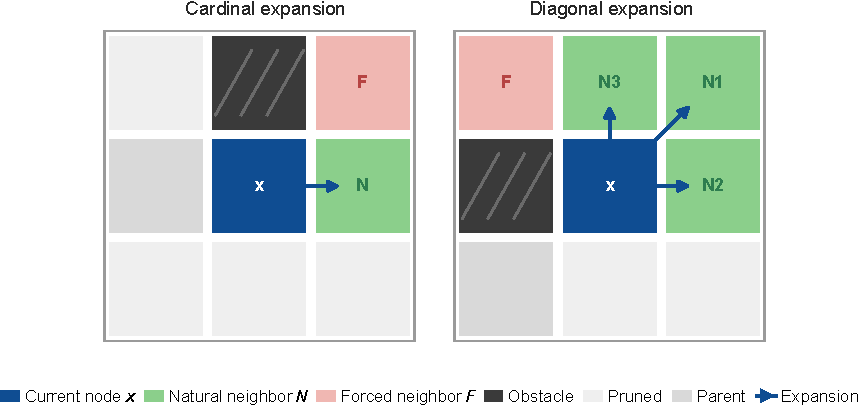
\includegraphics[width=3.0in]{figures/jps_pruning}
\caption{Illustration of the JPS neighbor-pruning rules.}
\label{fig:jps_pruning}
\end{figure}

Owing to the jumping nature of JPS, diagonal moves in the reconstructed path may cut across obstacle corners. To this end, the proposed algorithm detects such cases during path reconstruction and replaces the corresponding moves with L-shaped paths along the grid boundary, thereby avoiding collisions.

\subsubsection{Tie-Breaking Strategy}

When multiple nodes in the open set share the same $f$-value, the selection order of standard A* depends on the specific implementation (typically first-in-first-out or random) and is essentially arbitrary. However, among nodes with identical $f$-values, a node with a smaller $h$-value has a larger actual cost $g = f - h$, i.e., it lies farther from the start and closer to the goal. Expanding such nodes first steers the search toward the goal without affecting the optimality guarantee. Accordingly, the improved A* algorithm proposed in this paper adopts the tie-breaking rule ``when $f$-values are equal, prefer the node with the smaller $h$-value.'' The node comparison rule is defined as
\begin{equation}
\begin{cases}
n_1, & f(n_1) < f(n_2) \\
n_2, & f(n_1) > f(n_2) \\
n_1, & f(n_1) = f(n_2) \land h(n_1) < h(n_2) \\
n_2, & f(n_1) = f(n_2) \land h(n_1) > h(n_2)
\end{cases}
\label{eq:tbreak}
\end{equation}

In physical terms, the evaluation function $f(n) = g(n) + h(n)$ implies that when two nodes share the same $f$-value, the one with the larger $g$ is farther from the start, whereas the one with the smaller $h$ is closer to the goal. Prioritizing such nodes biases the search toward the goal and reduces ineffective exploration in regions away from the goal.

\subsection{Path Post-Processing}
\label{subsec:post}

The path obtained by JPS search consists of a sequence of grid-center points; it contains redundant intermediate points and is composed of discrete horizontal and vertical segments, resulting in insufficient smoothness. This section proposes a two-stage processing approach to resolve these issues.

\subsubsection{Safety-Aware Path Simplification}

Conventional path simplification methods, such as corner pruning, directly connect non-adjacent nodes on the path and skip intermediate points to reduce the number of path points. However, such methods typically only check whether the connecting segment crosses obstacles and ignore the safety margin between path points and obstacles; in obstacle-dense regions this may cause paths to pass excessively close to obstacles. To this end, this section proposes a safety-distance-aware path simplification algorithm, whose core idea is to maintain a minimum safety distance between the path and obstacles during simplification.

The algorithm processes the input path in a four-step procedure. First, the nodes at which the direction changes are identified from the path: while keeping the start and end points, the connection directions of each intermediate node with its predecessor and successor are computed, and nodes whose forward and backward connection directions differ are marked as corner points $C_i$. Second, starting from the current corner $C_i$, the subsequent corners $C_j$ ($j > i$) are scanned forward; each segment $C_i \to C_j$ is verified against the safety-distance constraint via the safety check, the intermediate corners are skipped, and the farthest reachable corner $j^{*}$ is recorded as the new anchor. This greedy strategy maximizes the single-step simplification while preserving safety. On this basis, after the greedy step determines the farthest reachable corner $j^{*}$, it checks whether a skipped corner $k$ ($i < k < j^{*}$) can reach a farther corner $j'$ ($j' > j^{*}$) directly via a safe segment; if so, the route $(k, j')$ is recorded. Subsequently, the lengths of the two routes are compared: route A has length $d(C_i, C_{j^{*}}) + d(C_{j^{*}}, C_{j'})$, i.e., reaching $j^{*}$ first and then continuing to $j'$; route B has length $d(C_i, C_k) + d(C_k, C_{j'})$, i.e., bypassing $j^{*}$ and routing through $k$. If route B is shorter, the intermediate corner $C_k$ is retained; otherwise, only the greedy result $C_{j^{*}}$ is kept. This comparison ensures that intermediate-corner exploration does not come at the cost of path efficiency. Algorithm~\textcolor{blue}{\ref{alg:simplify}} gives the pseudocode of the path simplification algorithm.

The safety-check function is implemented by dense cell-wise sampling: sample points are densely drawn along the segment from $p_1$ to $p_2$, and for each sample point its distance to the nearest obstacle-cell boundary is computed. If the distance of any sample point is smaller than the safety threshold $d_{\mathrm{safe}}$, the connection is deemed unsafe. The distance from a point to a cell boundary is given by
\begin{equation}
\begin{split}
d_x &= \max\left(0,\; |x_p - x_c| - 0.5\right)\\
d_y &= \max\left(0,\; |y_p - y_c| - 0.5\right)
\end{split}
\label{eq:dxymax}
\end{equation}

\begin{equation}
d(p, \mathrm{cell}) = \sqrt{d_x^2 + d_y^2}
\label{eq:dist}
\end{equation}
where $p = (x_p, y_p)$ is the sample point under the grid-to-continuous coordinate mapping described above, and $(x_c, y_c)$ is the center coordinate of the obstacle cell. The $\max(0, \cdot)$ operator handles the case in which the sample point has already fallen within the horizontal or vertical extent of the cell along a given axis. When the computed distance $d(p, \mathrm{cell})$ is smaller than the set safety-distance threshold $d_{\mathrm{safe}}$, the sample point has entered the safety exclusion zone of the obstacle cell.

\begin{algorithm}[!t]
\caption{Safety-distance-aware path simplification}
\label{alg:simplify}
\begin{spacing}{0.9}
\begin{algorithmic}[1]
\REQUIRE grid path $P = [P_1, \ldots, P_N]$, occupancy grid, safety margin $d_{\mathrm{safe}}$
\ENSURE simplified path $P_s$ ($|P_s| \leq N$)
\STATE $C \gets$ the corner points of $P$ where the direction changes, plus the two endpoints;
\STATE $P_s \gets [C_1]$; $\; i \gets 1$;
\WHILE{$i < |C|$}
\STATE $j^{*} \gets$ the farthest corner reachable from $C_i$ by a collision-free segment; \quad\textit{greedy forward scan}
\IF{$j^{*} = |C|$}
\STATE append $C_{|C|}$ to $P_s$ and break;
\ENDIF
\STATE $(k^{*}, j') \gets$ among all skipped corners $k$ ($i < k < j^{*}$) and farther corners $j$ ($j^{*} < j \leq |C|$), the pair with the largest $j$ such that the segment $C_k \to C_j$ is collision-free;
\IF{$k^{*}$ exists and $d(C_i, C_{k^{*}}) + d(C_{k^{*}}, C_{j'}) < d(C_i, C_{j^{*}}) + d(C_{j^{*}}, C_{j'})$}
\STATE append $C_{k^{*}}$ and $C_{j'}$ to $P_s$, and set $i \gets j'$; \quad\textit{route through the intermediate corner}
\ELSE
\STATE append $C_{j^{*}}$ to $P_s$, and set $i \gets j^{*}$;
\ENDIF
\ENDWHILE
\RETURN $P_s$;
\end{algorithmic}
\end{spacing}
\end{algorithm}

\subsubsection{Arc-Length Parameterized Cubic Spline Smoothing}

Although the simplified path has removed redundant points, the output path is not sufficiently smooth and can hardly reflect the actual traveled distance of the motion. To this end, this paper adopts arc-length parameterized cubic spline smoothing, using the cumulative Euclidean distance between path points rather than the point index as the parameter, so that the parameter space remains consistent with the actual geometric space. The first step of the smoothing process is densification of sparse segments: for sparse segments whose adjacent points are separated by more than 2 grid units, $\lfloor \ell / 2 \rfloor$ intermediate points are linearly interpolated along the segment between the two endpoints. The purpose of densification is to provide the spline with sufficient control points and to prevent the Runge phenomenon on long straight segments caused by an insufficient number of control points, which would otherwise cause the curve to deviate from the intended polyline or even clip obstacle corners. The second step is arc-length parameterization. Let the densified path-point sequence be $\{P_0, P_1, \ldots, P_M\}$, where $P_i = (x_i, y_i)$ are continuous coordinates. The cumulative chord-length parameters are computed as $s_0 = 0$ and $s_i = s_{i-1} + \|P_i - P_{i-1}\|_2$ ($i = 1, 2, \ldots, M$). Cubic spline interpolation is then performed for $x(s)$ and $y(s)$ separately with $s$ as the independent variable, yielding the parametric curve $(x(s), y(s))$. On each subinterval $[s_i, s_{i+1}]$, the cubic spline is a cubic polynomial that guarantees continuity of the first- and second-order derivatives, and hence continuity of the curve curvature. The third step is equal arc-length resampling. The final smoothed path-point sequence is generated by uniformly sampling along the arc-length parameter $s$ at an interpolation density $\rho$. Because $s$ is approximately linearly related to the actual geometric distance, equal arc-length sampling ensures a uniform spatial distribution of path points and avoids the problem of conventional equal-parameter sampling, which places points densely at high curvature and sparsely at low curvature. Algorithm~\textcolor{blue}{\ref{alg:smooth}} gives the pseudocode of the smoothing algorithm.

\begin{algorithm}[!t]
\caption{Arc-length parameterized cubic spline smoothing}
\label{alg:smooth}
\begin{spacing}{0.9}
\begin{algorithmic}[1]
\REQUIRE grid path $P = [P_1, \ldots, P_N]$, density $\rho$ (default $10$)
\ENSURE smoothed continuous path $Q = [Q_1, \ldots, Q_M]$ in $[x, y]$
\STATE convert each grid point $P_i = (r_i, c_i)$ to continuous coordinates $(x_i, y_i) = (c_i - 0.5,\; r_i - 0.5)$;
\FOR{each consecutive pair whose segment length exceeds $2$}
\STATE insert $\lfloor \mathrm{length} / 2 \rfloor$ equally spaced intermediate points along the segment; \quad\textit{densification to prevent spline overshoot}
\ENDFOR
\STATE compute the cumulative chord length $t_1 = 0$, $t_i = t_{i-1} + \|P_i - P_{i-1}\|_2$; \quad\textit{arc-length parameter}
\STATE remove duplicate $t$ values to keep strict monotonicity;
\STATE fit cubic splines $x(t)$ and $y(t)$ through the densified points;
\STATE sample $x(t)$ and $y(t)$ at $\rho$ points per segment to obtain $Q$;
\RETURN $Q$;
\end{algorithmic}
\end{spacing}
\end{algorithm}

\subsubsection{Pipeline Integration}

The above post-processing operations are integrated as a pipeline: the JPS search outputs the raw grid path $\to$ SimplifyPath removes redundant points $\to$ SmoothPath generates a smooth continuous-coordinate path. The entire pipeline is completed in one pass, and the resulting path possesses both a safety margin and smoothness. The rationale of this two-stage design is that path simplification and spline smoothing address two distinct dimensions of path quality. Safety-aware path simplification reduces the number of path points and lowers the complexity of subsequent computation while guaranteeing the safety margin of the path; smoothing converts the discrete grid path into a continuous curve, enabling the robot to track the path with a smooth motion trajectory. If smoothing is applied without prior simplification, the spline must handle a large number of redundant control points, which not only increases computational cost but may also produce unstable curve shapes due to excessively dense control points. A comparison of the path before and after post-processing is shown in Fig.~\textcolor{blue}{\ref{fig:pipeline}}.

\begin{figure}[!t]
\centering
\subfloat[Original path and simplified path]{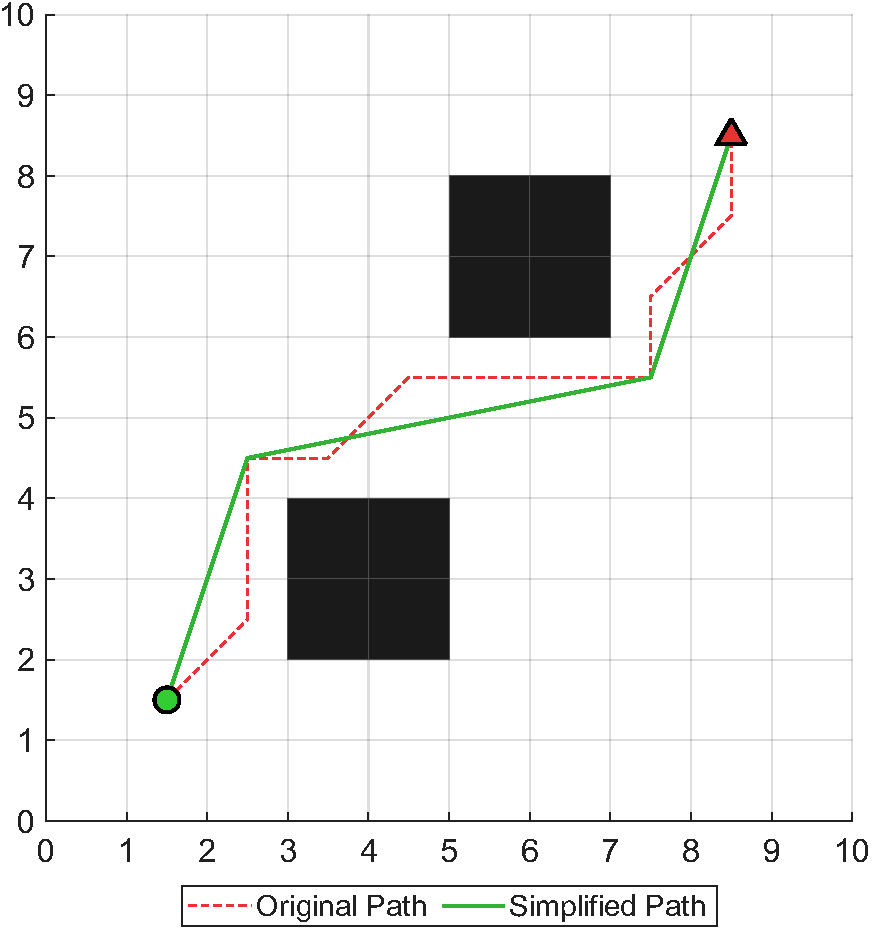
\includegraphics[width=1.55in]{figures/SimplifyPath}%
\label{fig:pipeline_a}}%
\hfil
\subfloat[Simplified path and smoothed path]{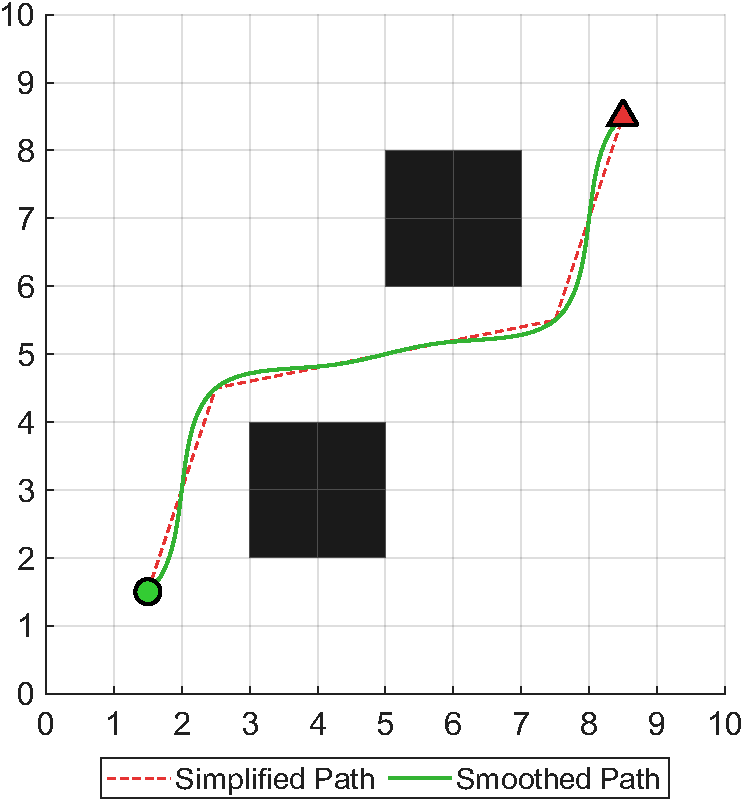
\includegraphics[width=1.55in]{figures/SmoothPath}%
\label{fig:pipeline_b}}
\caption{Comparison of the path at the individual stages of the pipeline.}
\label{fig:pipeline}
\end{figure}
